%=-=-=-=-=-=-=-=-=-=-=-=-=-=-=-=-=-=-=-=-=-=-=-=-=-=-=-=-=-=-=-=-=-=- CHAPTER 03
\chapter{Figures \& Images}

%=-=-=-=-=-=-=-=-=-=-=-=-=-=-=-=-=-=-=-=-=-=-=-=-=-=-=-=-=-=-=-=-=-=-=-= SECTION
\section{Storing Images}

Images can be easily included in your document by using the \cs{includegraphics}
macro included with the graphics package. Before we include our first image, we 
should probably create a folder to hold all our images to keep our directory 
lean in terms of the number of files.  My personal preference is to keep my 
images in the folder called \verb!~/assets!, which is relative to the directory
of my main file.  Rather than have to provide the path of where your images are 
located there is a \cs{graphicspath} macro that you can place in the preamble
that allows you to assign one or more locations for \LaTeX ~to look for image 
files.
\begin{dispListing}
\graphicspath{{/assets/}}
\end{dispListing}
Or if you have more than one directory
\begin{dispListing}
\graphicspath{{/assets/}{/images/}{/pdfs/}}
\end{dispListing}
This will save you a lot of extra typing and worry about where your images are
being stored.

%=-=-=-=-=-=-=-=-=-=-=-=-=-=-=-=-=-=-=-=-=-=-=-=-=-=-=-=-=-=-=-=-=-=-=-= SECTION
\section{Including Images}

To include an image we will be using the \cs{includegraphics} macro, which accepts 
the path and file name as its argument and can take multiple options.  If you made
use of the \cs{graphicspath} macro, made available by default for this template, 
then the argument is the file name.  The file extension is optional, unless you 
have multiple files with the same name, but with different extensions.  Let's 
scale an image such that it's width is a quarter of the textwidth and center 
it by placing it in a center environment.
\begin{dispExample}
\begin{center}
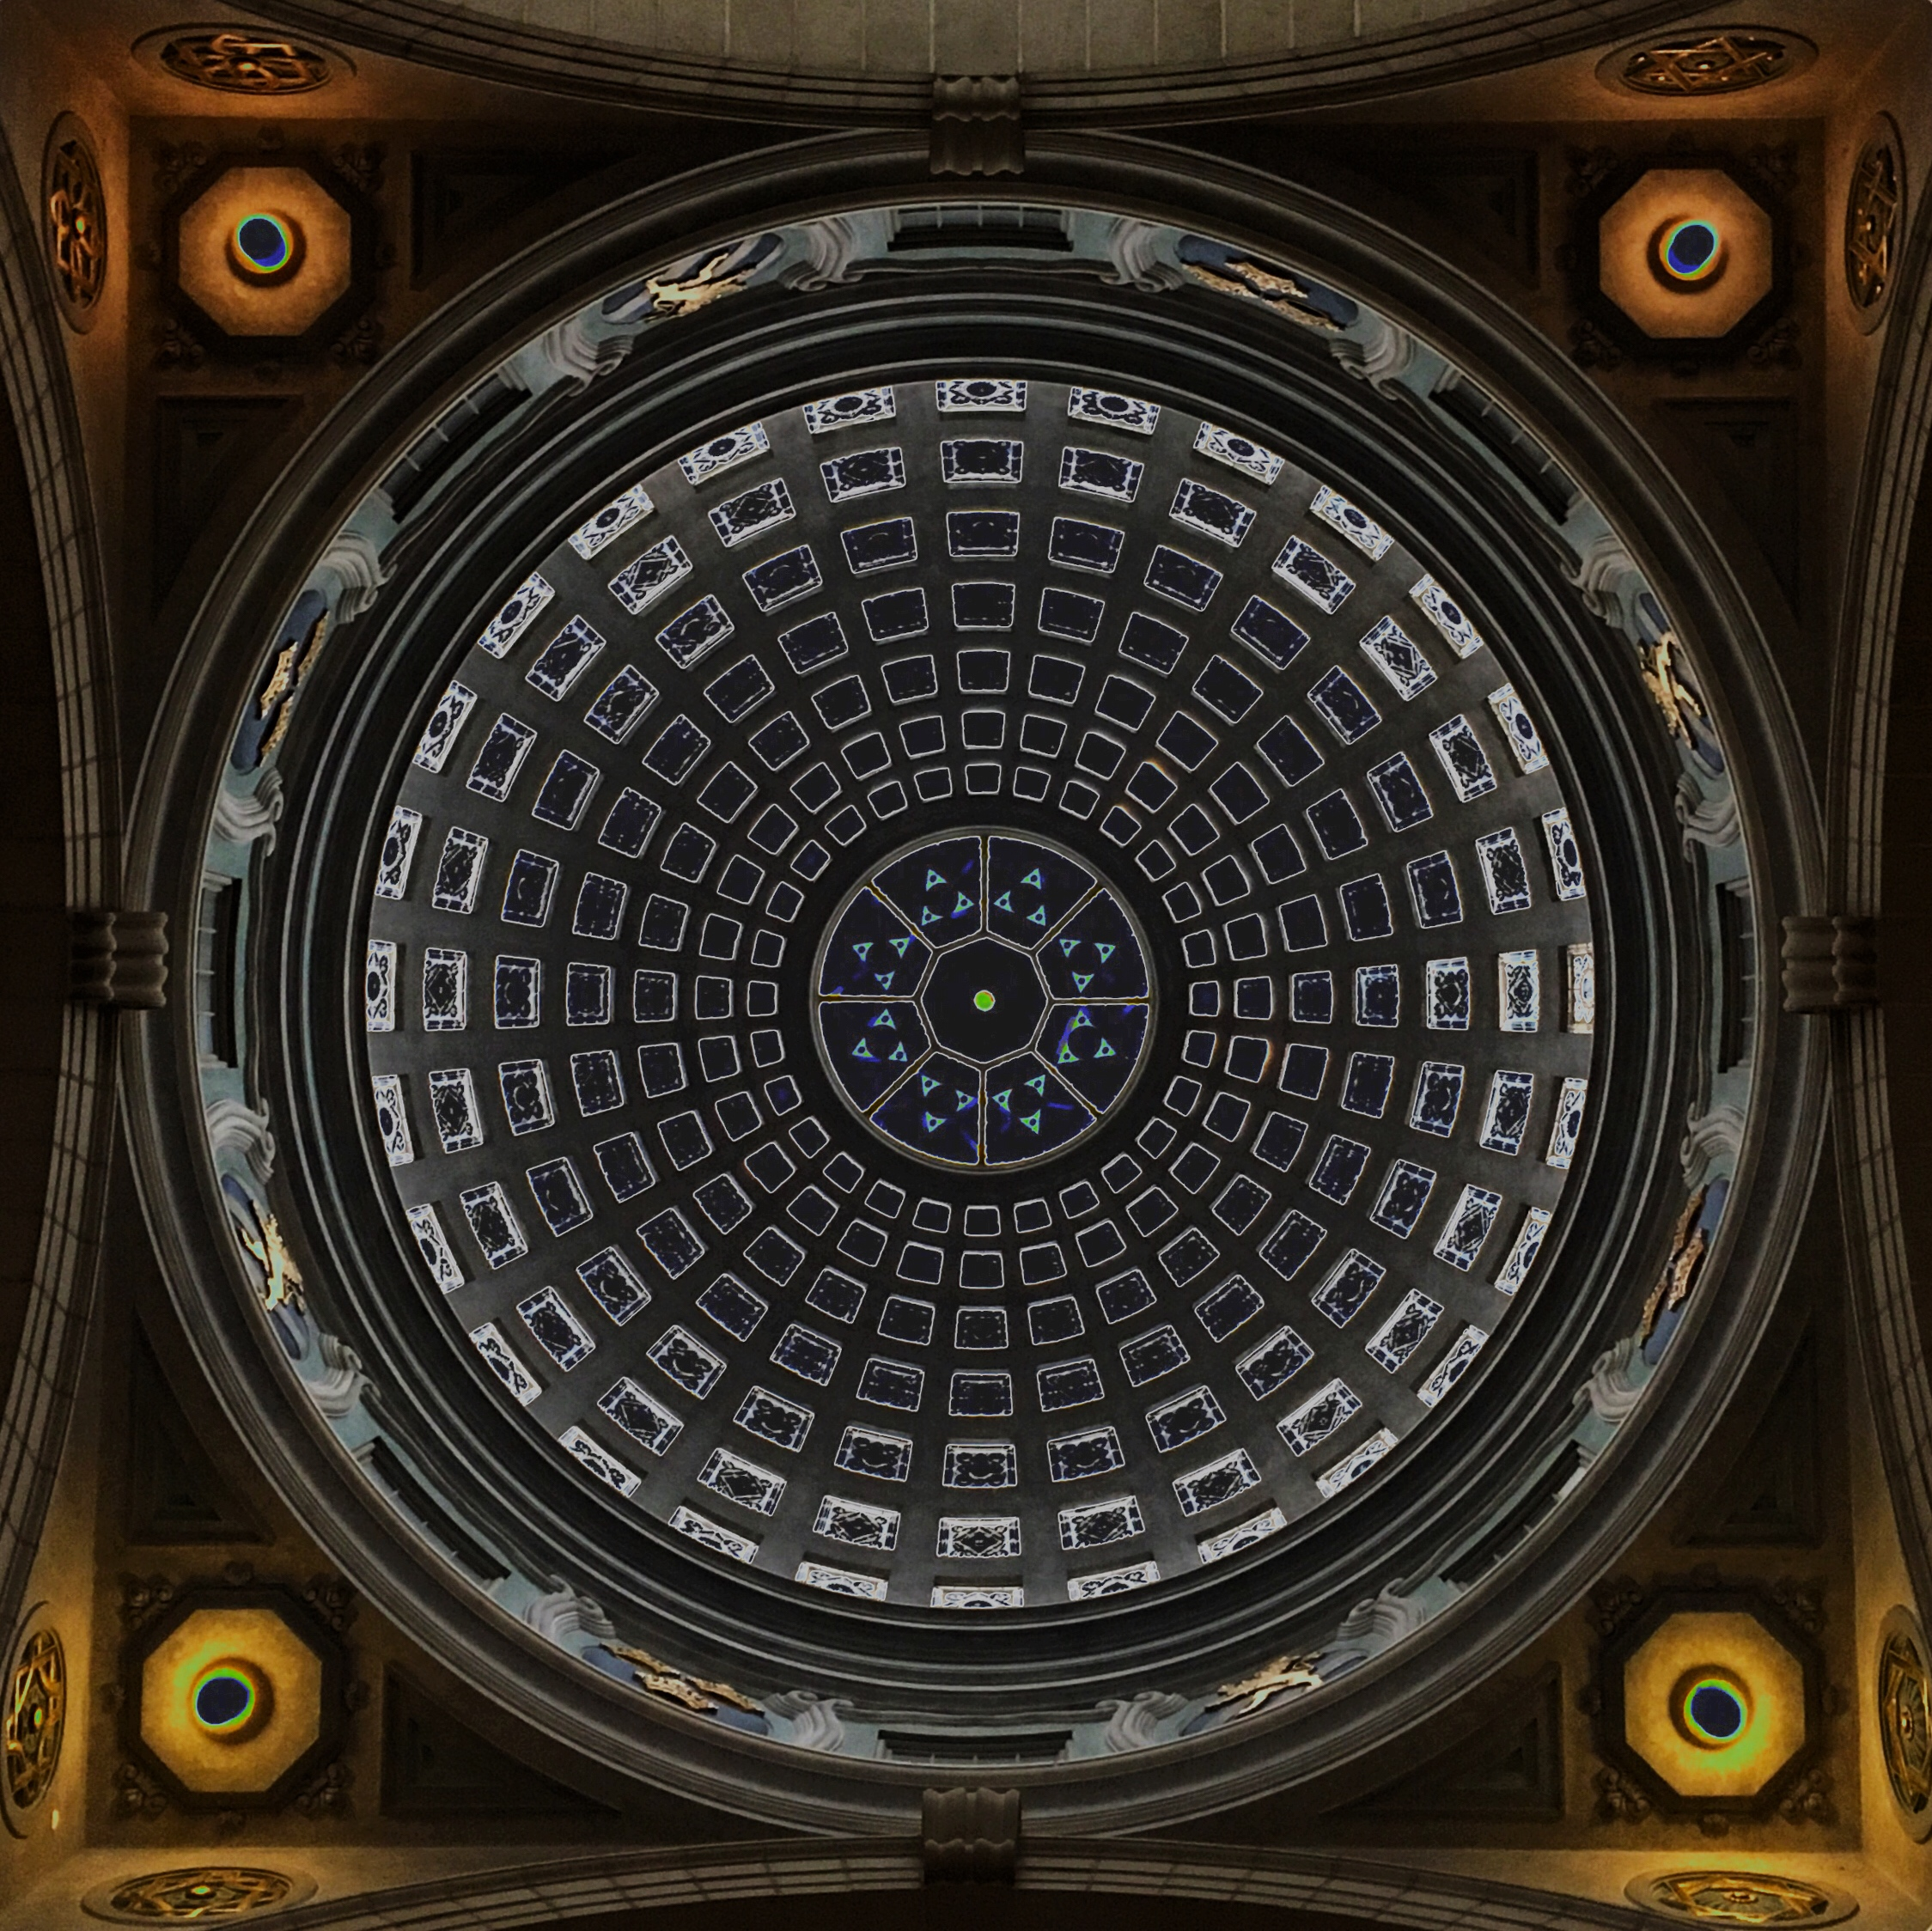
\includegraphics[width = 0.25\textwidth]{image.jpg}
\end{center}
\end{dispExample}


%=-=-=-=-=-=-=-=-=-=-=-=-=-=-=-=-=-=-=-=-=-=-=-=-=-=-=-=-=-=-=-=-=-=-=-= SECTION
\section{Figure Environment}
You will probably want to reference your image at some point in your text and
will most likely want to provide it with a caption.  For this we are going to
use the figure environment, which will calculate the best position to place 
your image within the document.  Don't worry, there are ways to manually place 
the image where you would like it to appear.
\begin{docEnvironment}[doclang/environment content=image content goes here]{figure}{\oarg{h, t}}{}
    \begin{dispListing}
        \begin{center}
        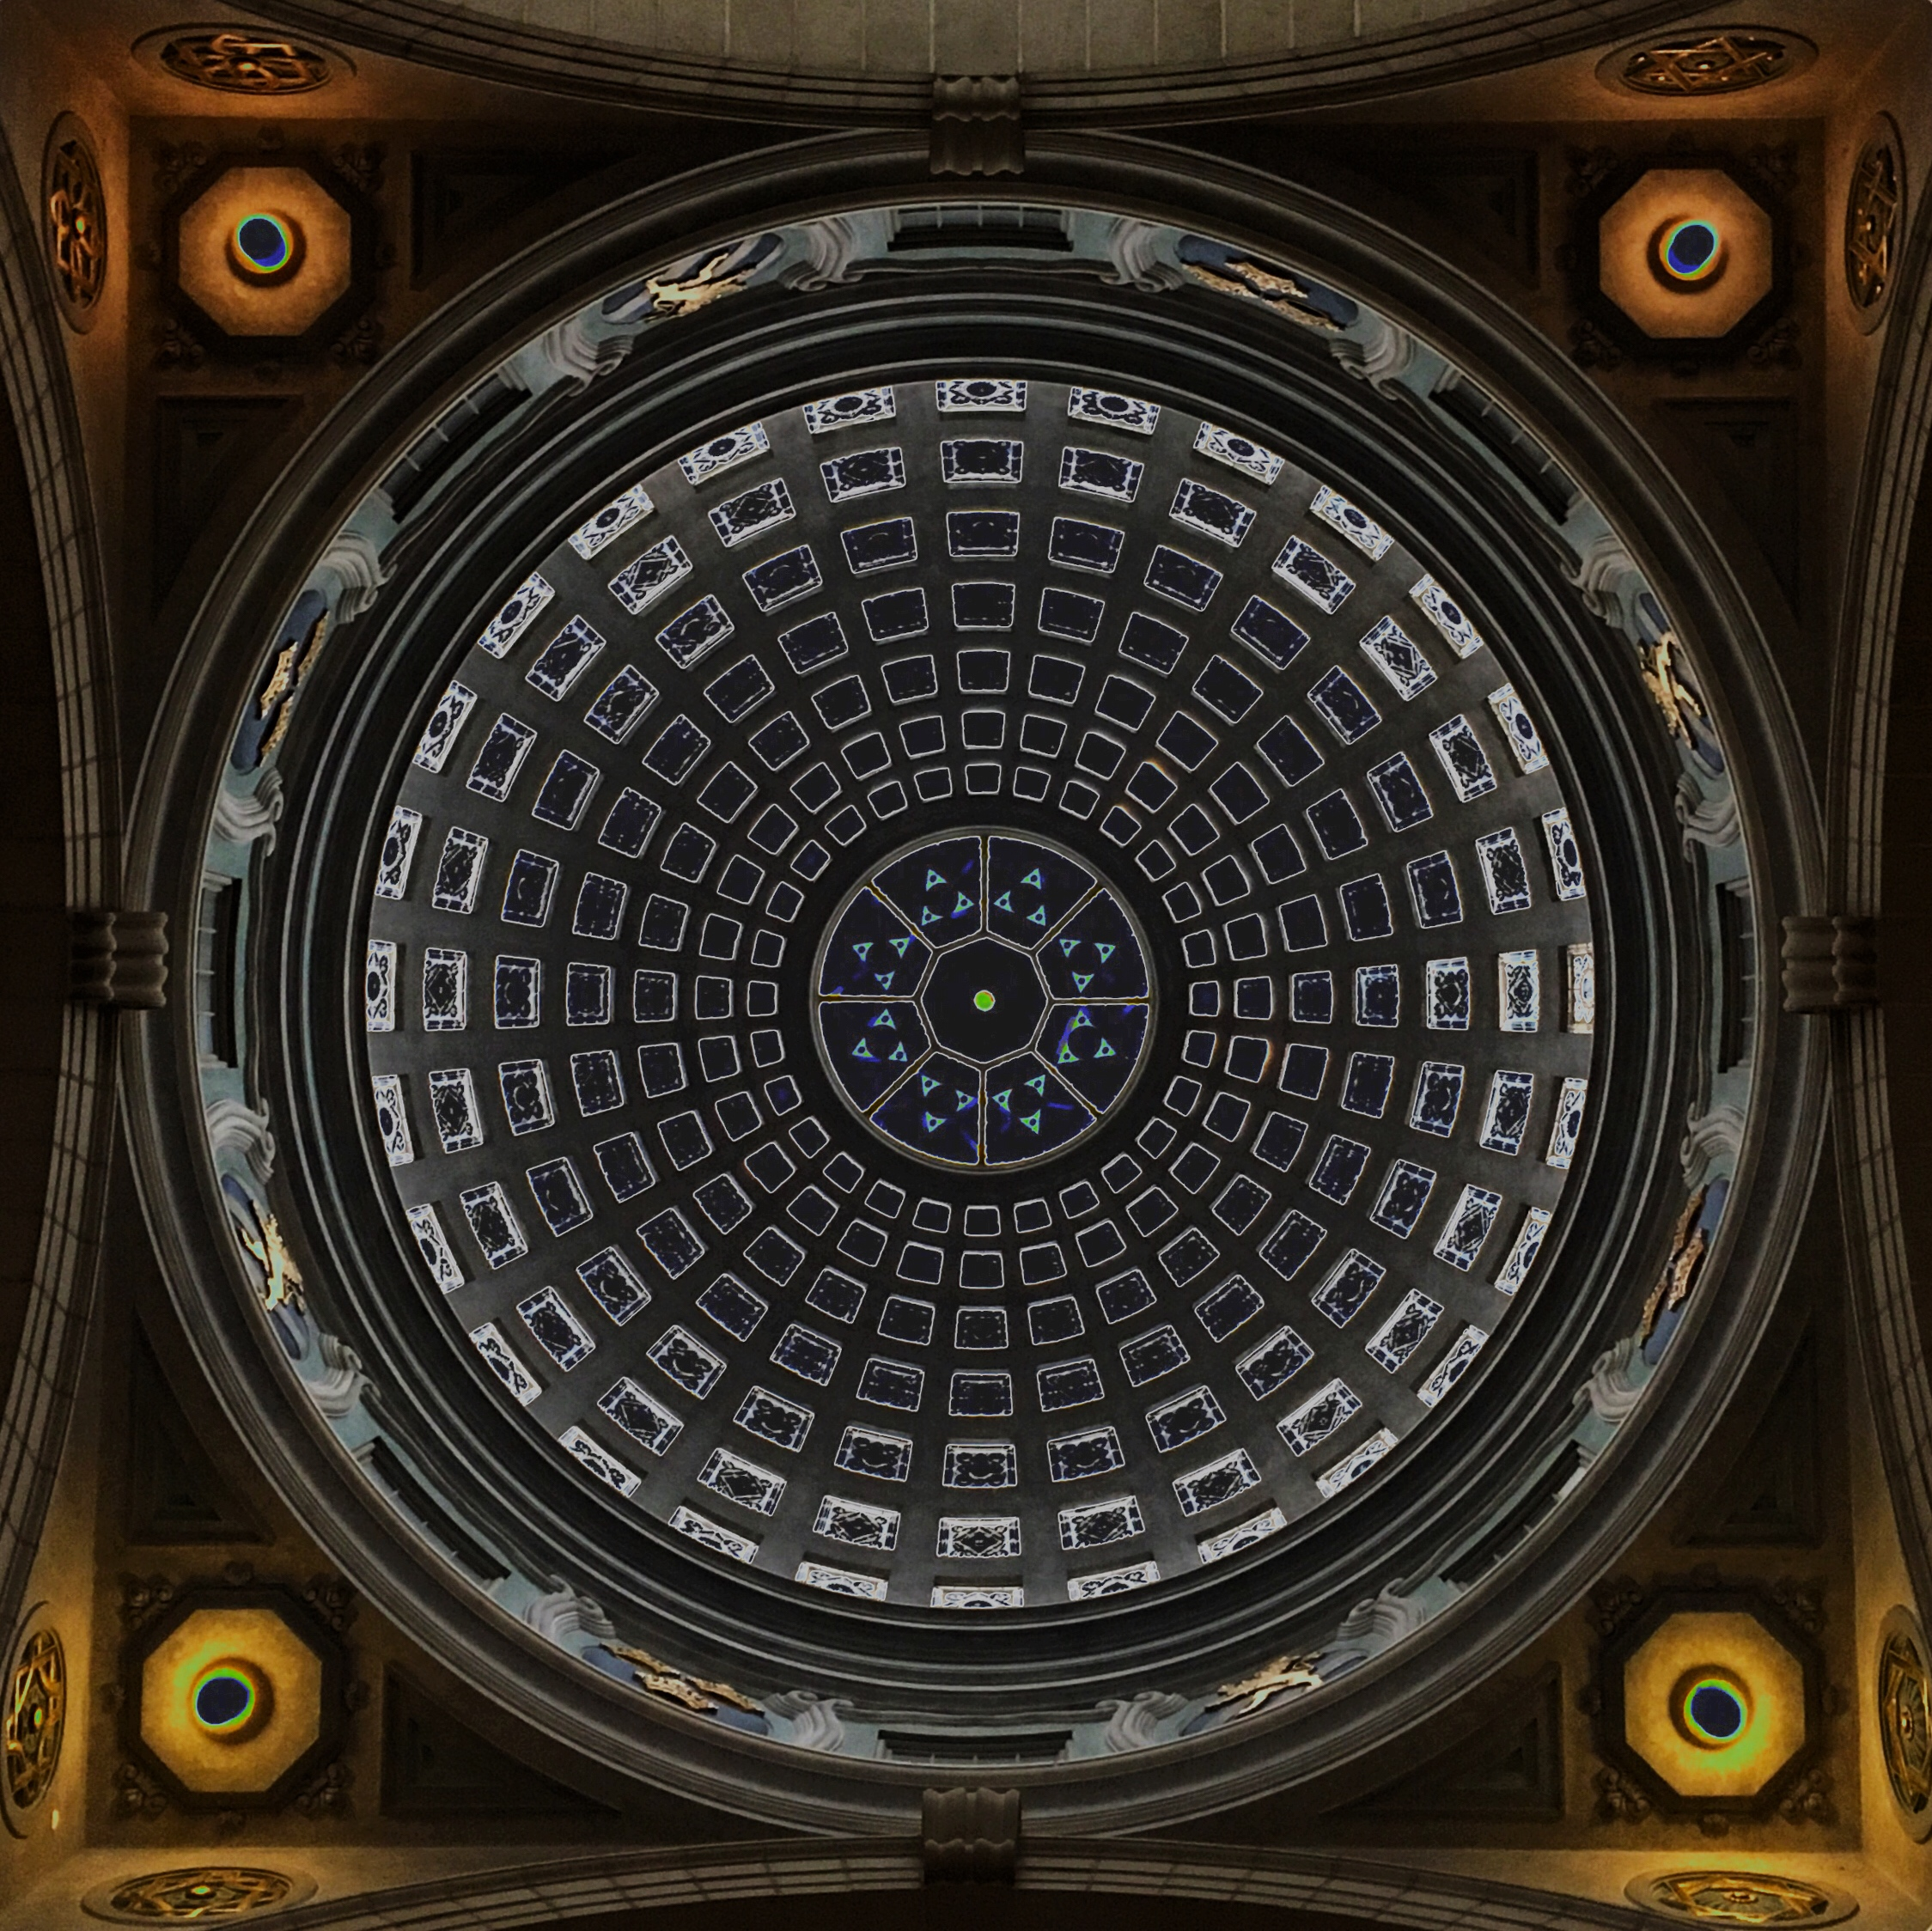
\includegraphics[width = 0.25\textwidth]{image.jpg}
        \end{center}
        \caption{Here is my excellent image.}
        \label{fig:img###}
        \end{dispListing}
\end{docEnvironment}
\begin{figure}[h]
    \begin{center}
    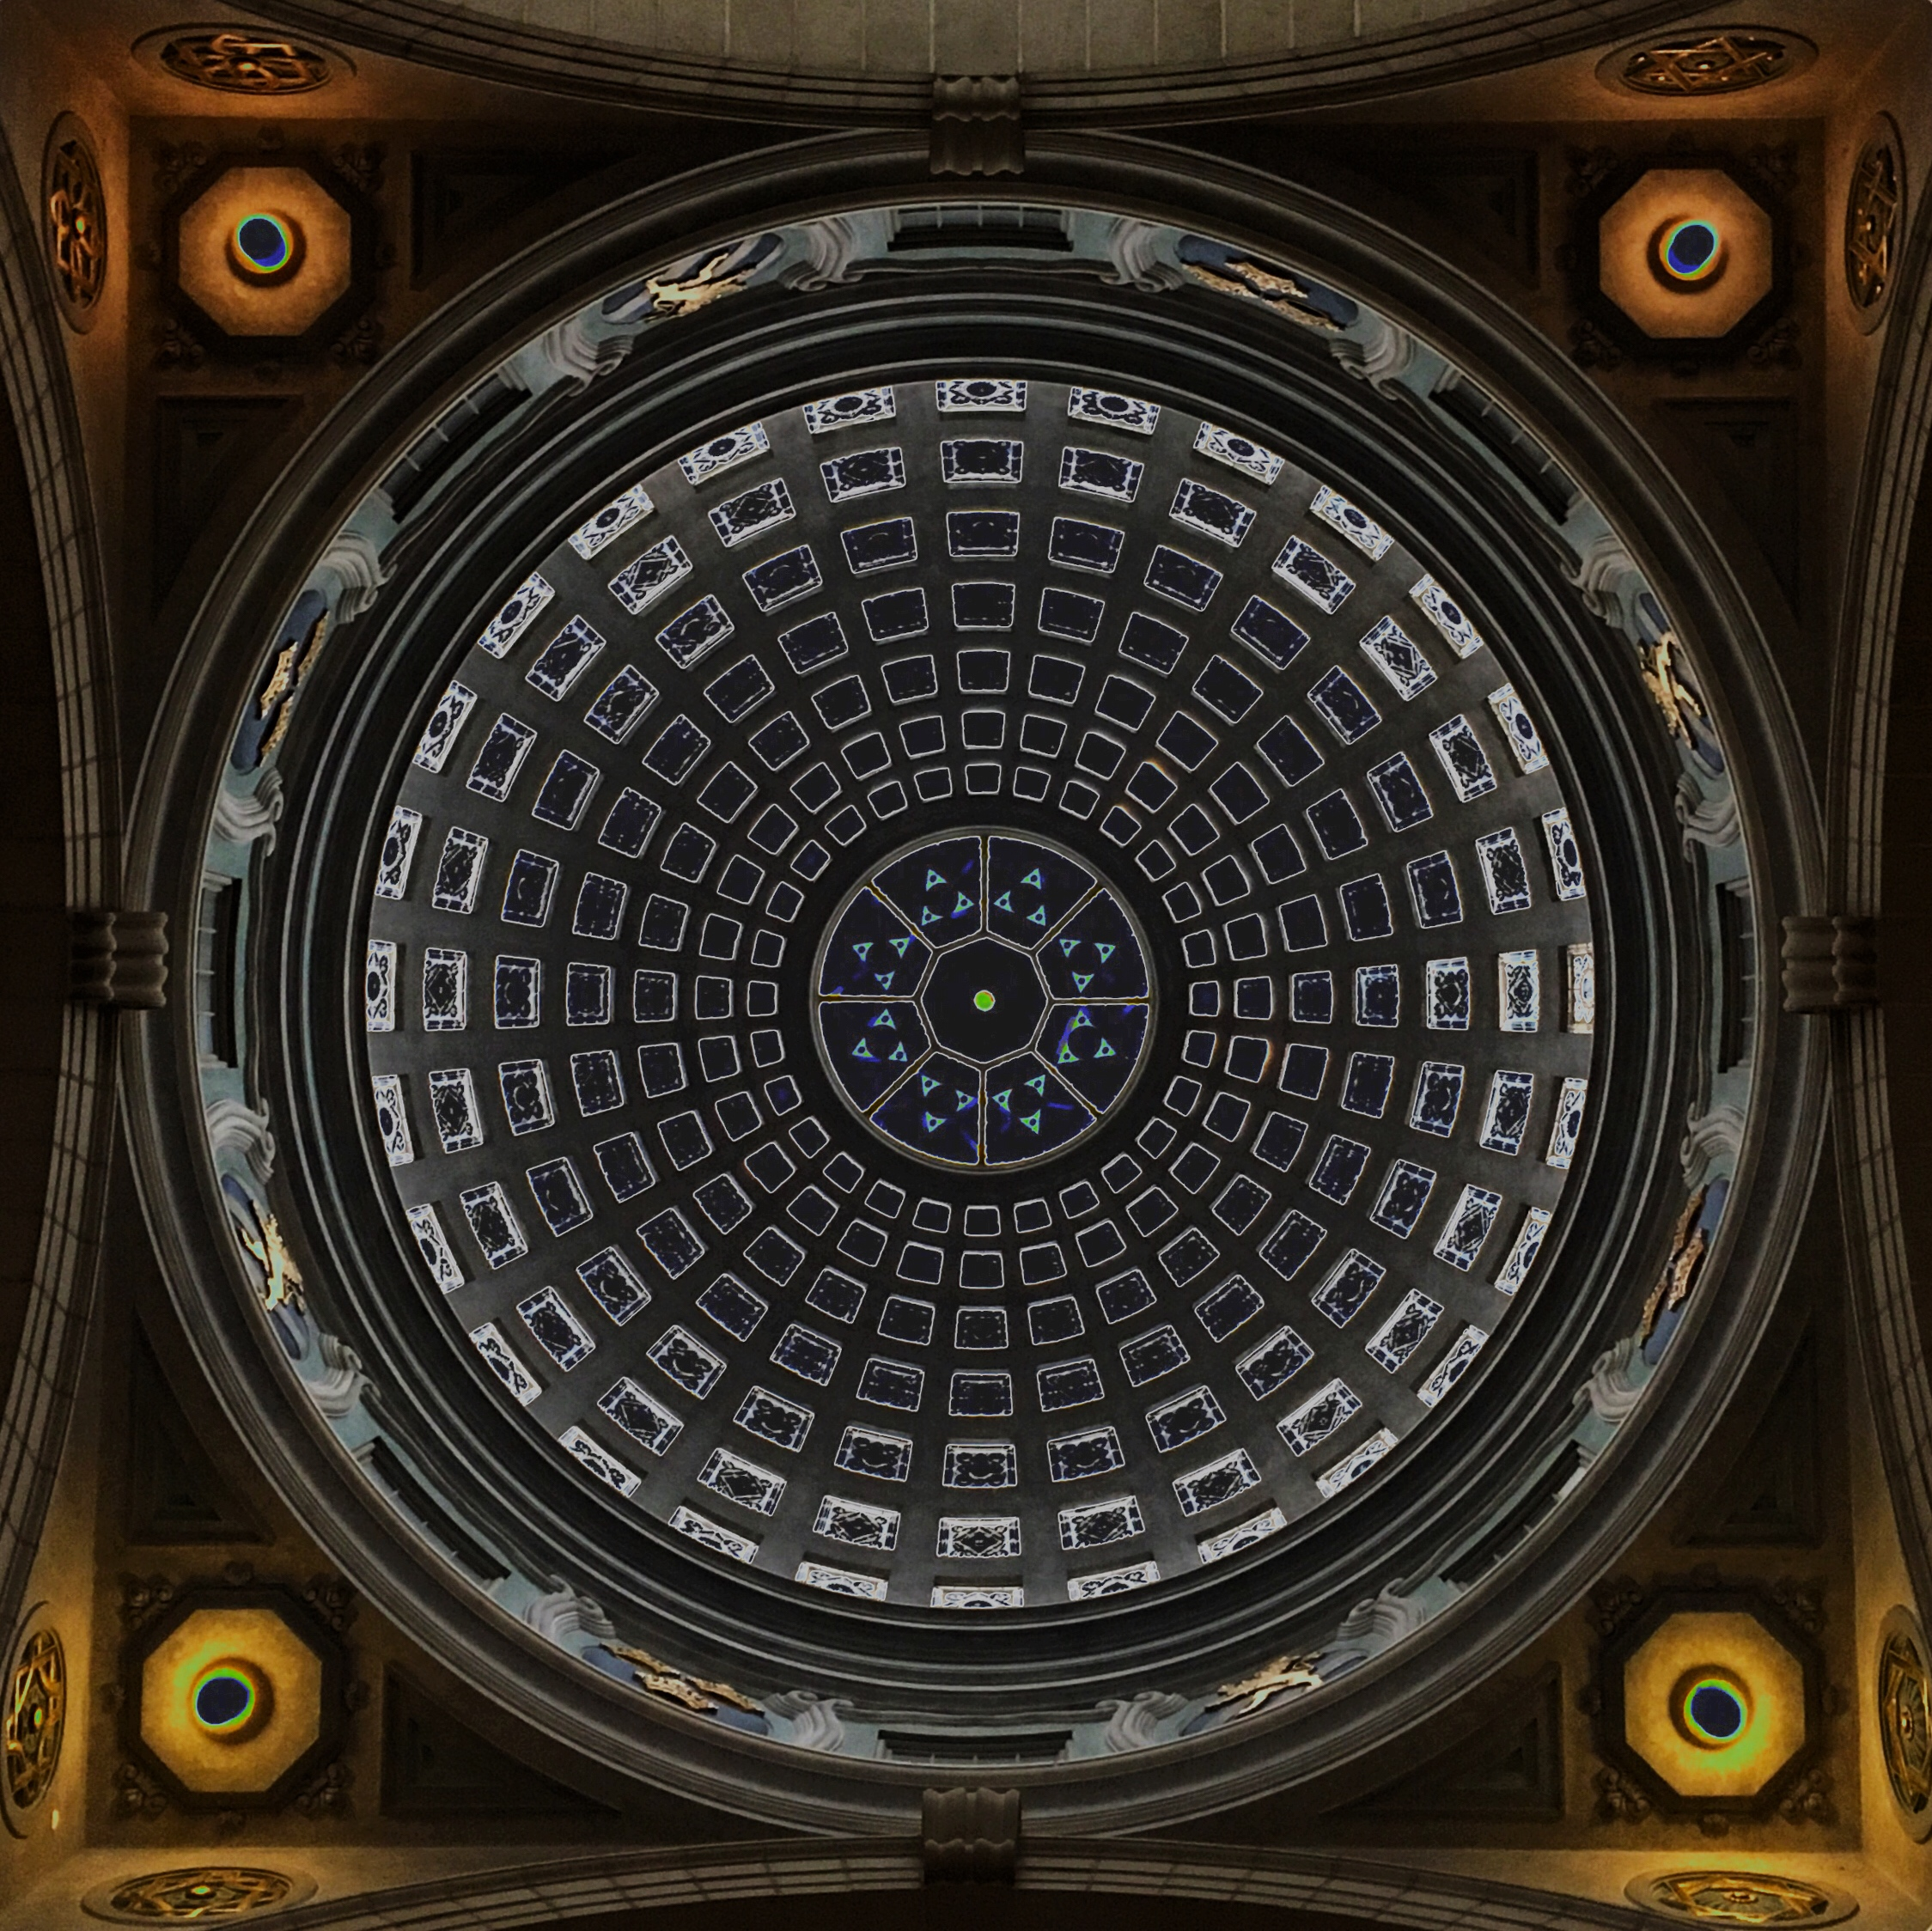
\includegraphics[width = 0.5\textwidth]{image.jpg}
    \end{center}
    \caption{Here is my excellent image.}
    \label{fig:img001}
\end{figure}
This would generate figure \ref{fig:img001}.

%=-=-=-=-=-=-=-=-=-=-=-=-=-=-=-=-=-=-=-=-=-=-=-=-=-=-=-=-=-=-=-=-=-=-=-= SECTION
\section{Multiple Horizontally Aligned Images}

Quite often it is the case that we want to include multiple horizontally
aligned images.  The figure environment is not well equipped for this task, so
we care going to make use of the subfigure package which will give us the 
subfigure environment that we can embed in our figure environment.  This will
enable us to assign both a caption and a label to each image separately.
\begin{docEnvironment}[doclang/environment content=image content goes here]{subfigure}{}{}
\begin{dispListing}
\begin{figure}
    \begin{center}
    \begin{subfigure}[b]{0.3\textwidth}
        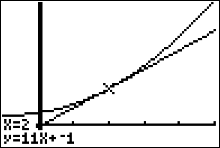
\includegraphics[width=\textwidth]{20170509-123642}
        \caption{Step 1}
        \label{fig:step1a}
    \end{subfigure}
    ~   % > > > Add desired spacing between images, e. g. ~, \quad, \qquad,
                % \hfill etc. (or a blank line to force the subfigure onto
                % a new line)
    \begin{subfigure}[b]{0.3\textwidth}
        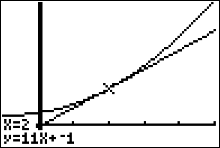
\includegraphics[width=\textwidth]{20170509-123642.png}
        \caption{Step 2}
        \label{fig:step2a}
    \end{subfigure}
    ~   % > > > Add desired spacing between images, e. g. ~, \quad, \qquad,
                % \hfill etc. (or a blank line to force the subfigure onto
                % a new line)
    \begin{subfigure}[b]{0.3\textwidth}
        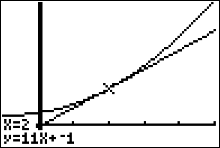
\includegraphics[width=\textwidth]{20170509-123642.png}
        \caption{Step 3}
        \label{fig:step3a}
    \end{subfigure}
    \caption{The Steps Shown}\label{fig:threestepsa}
    \end{center}
\end{figure}
\end{dispListing}
\end{docEnvironment}
\begin{figure}
    \begin{center}
    \begin{subfigure}[b]{0.3\textwidth}
        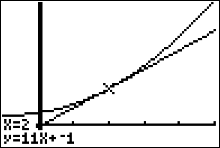
\includegraphics[width=\textwidth]{20170509-123642}
        \caption{Step 1}
        \label{fig:step1}
    \end{subfigure}
    ~   % > > > Add desired spacing between images, e. g. ~, \quad, \qquad,
                % \hfill etc. (or a blank line to force the subfigure onto
                % a new line)
    \begin{subfigure}[b]{0.3\textwidth}
        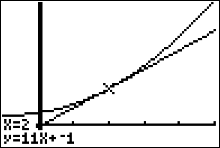
\includegraphics[width=\textwidth]{20170509-123642.png}
        \caption{Step 2}
        \label{fig:step2}
    \end{subfigure}
    ~   % > > > Add desired spacing between images, e. g. ~, \quad, \qquad,
                % \hfill etc. (or a blank line to force the subfigure onto
                % a new line)
    \begin{subfigure}[b]{0.3\textwidth}
        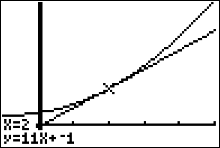
\includegraphics[width=\textwidth]{20170509-123642.png}
        \caption{Step 3}
        \label{fig:step3}
    \end{subfigure}
    \caption{The Steps Shown}\label{fig:threesteps}
    \end{center}
\end{figure}